\clearpage

\section{Brief History of Information Visualization}\label{sec:history-information-visualization}

%See \Cref{sec:information-visualization} for information about how we do this.
We use information visualization techniques to present data visually so that it is easier for people to understand it.
Throughout history, various ways of representing all kinds of data have been tried and developed. Some of the most
important and most used ones include tables, pie charts, bar charts, histograms, box and whisker plots, scatter plots, etc.

The first documented instance of a graph of statistical data is a 1644 graph by Michael Florent van Langren~\citep{friendly2010first}.
This one-dimensional line graph represents the twelve estimations of the difference in longitude between Toledo and
Rome and the names of astronomers who made the estimation.

\begin{figure}[h]
    \begin{center}
        % Vidiš ovo 0.5\textwidth je postotak širine stranice. ili samo \textwidth ako ćeš čitavom širinom
        %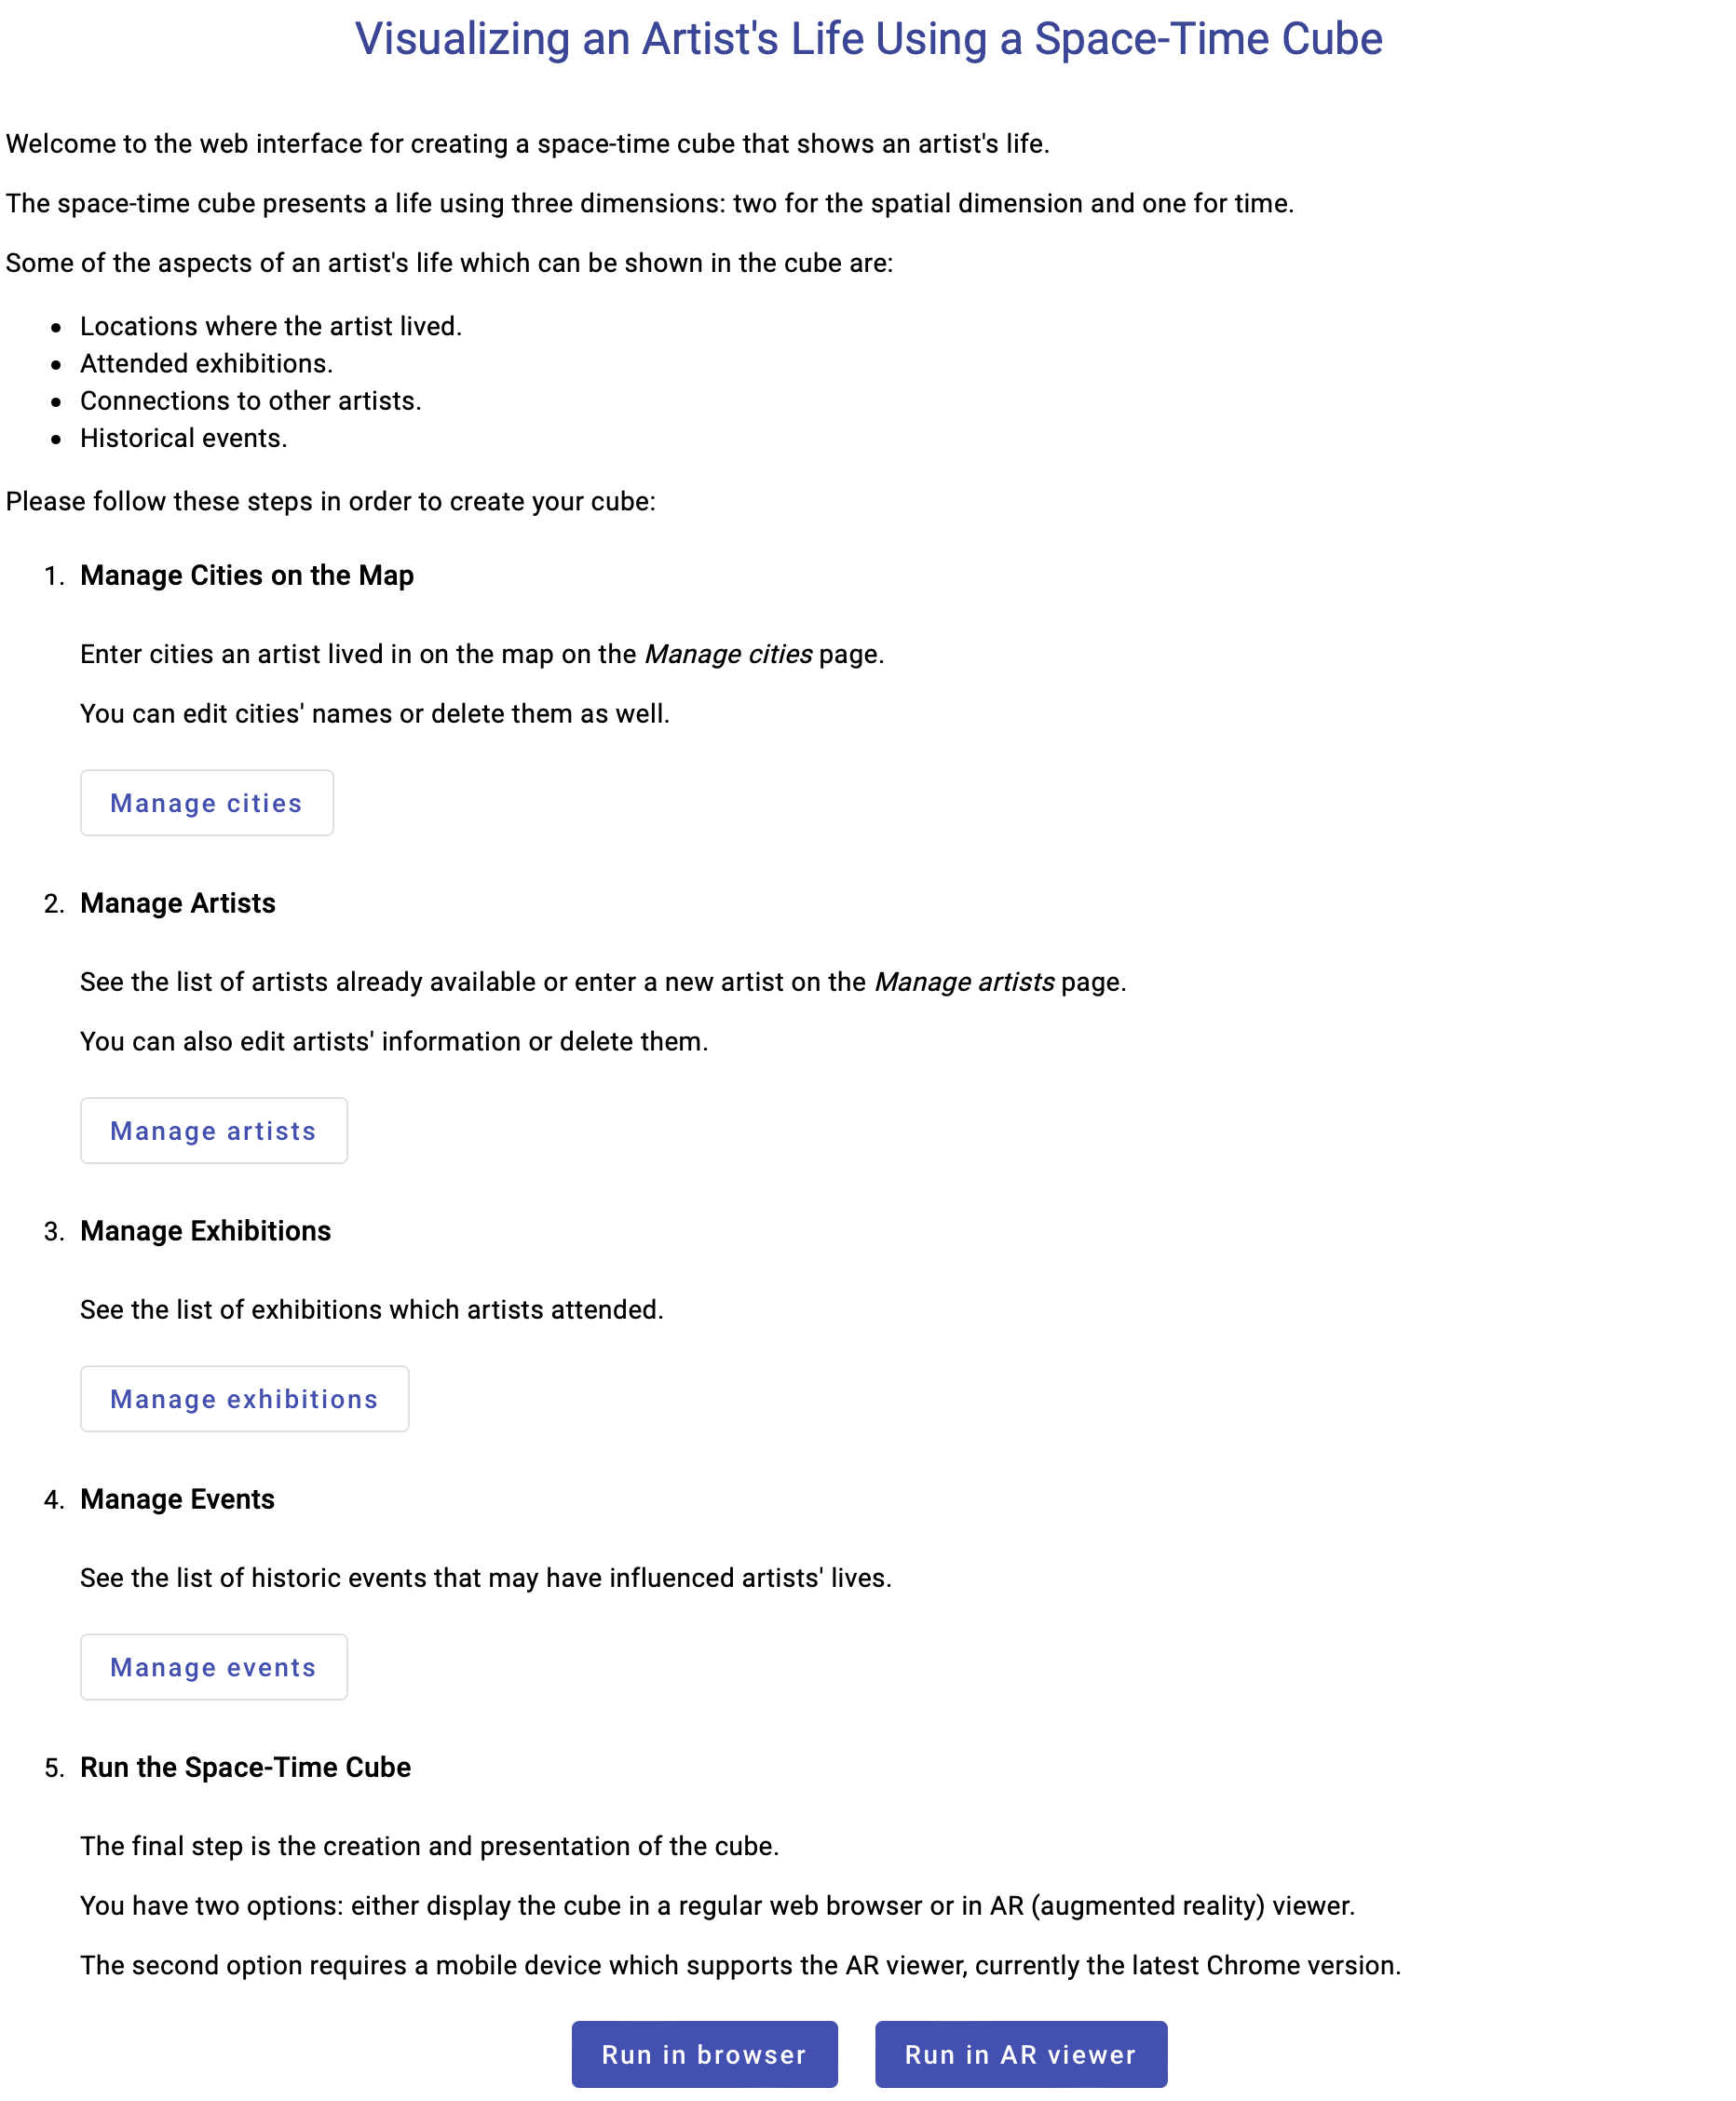
\includegraphics[width=0.5\textwidth]{graphics/1}
        %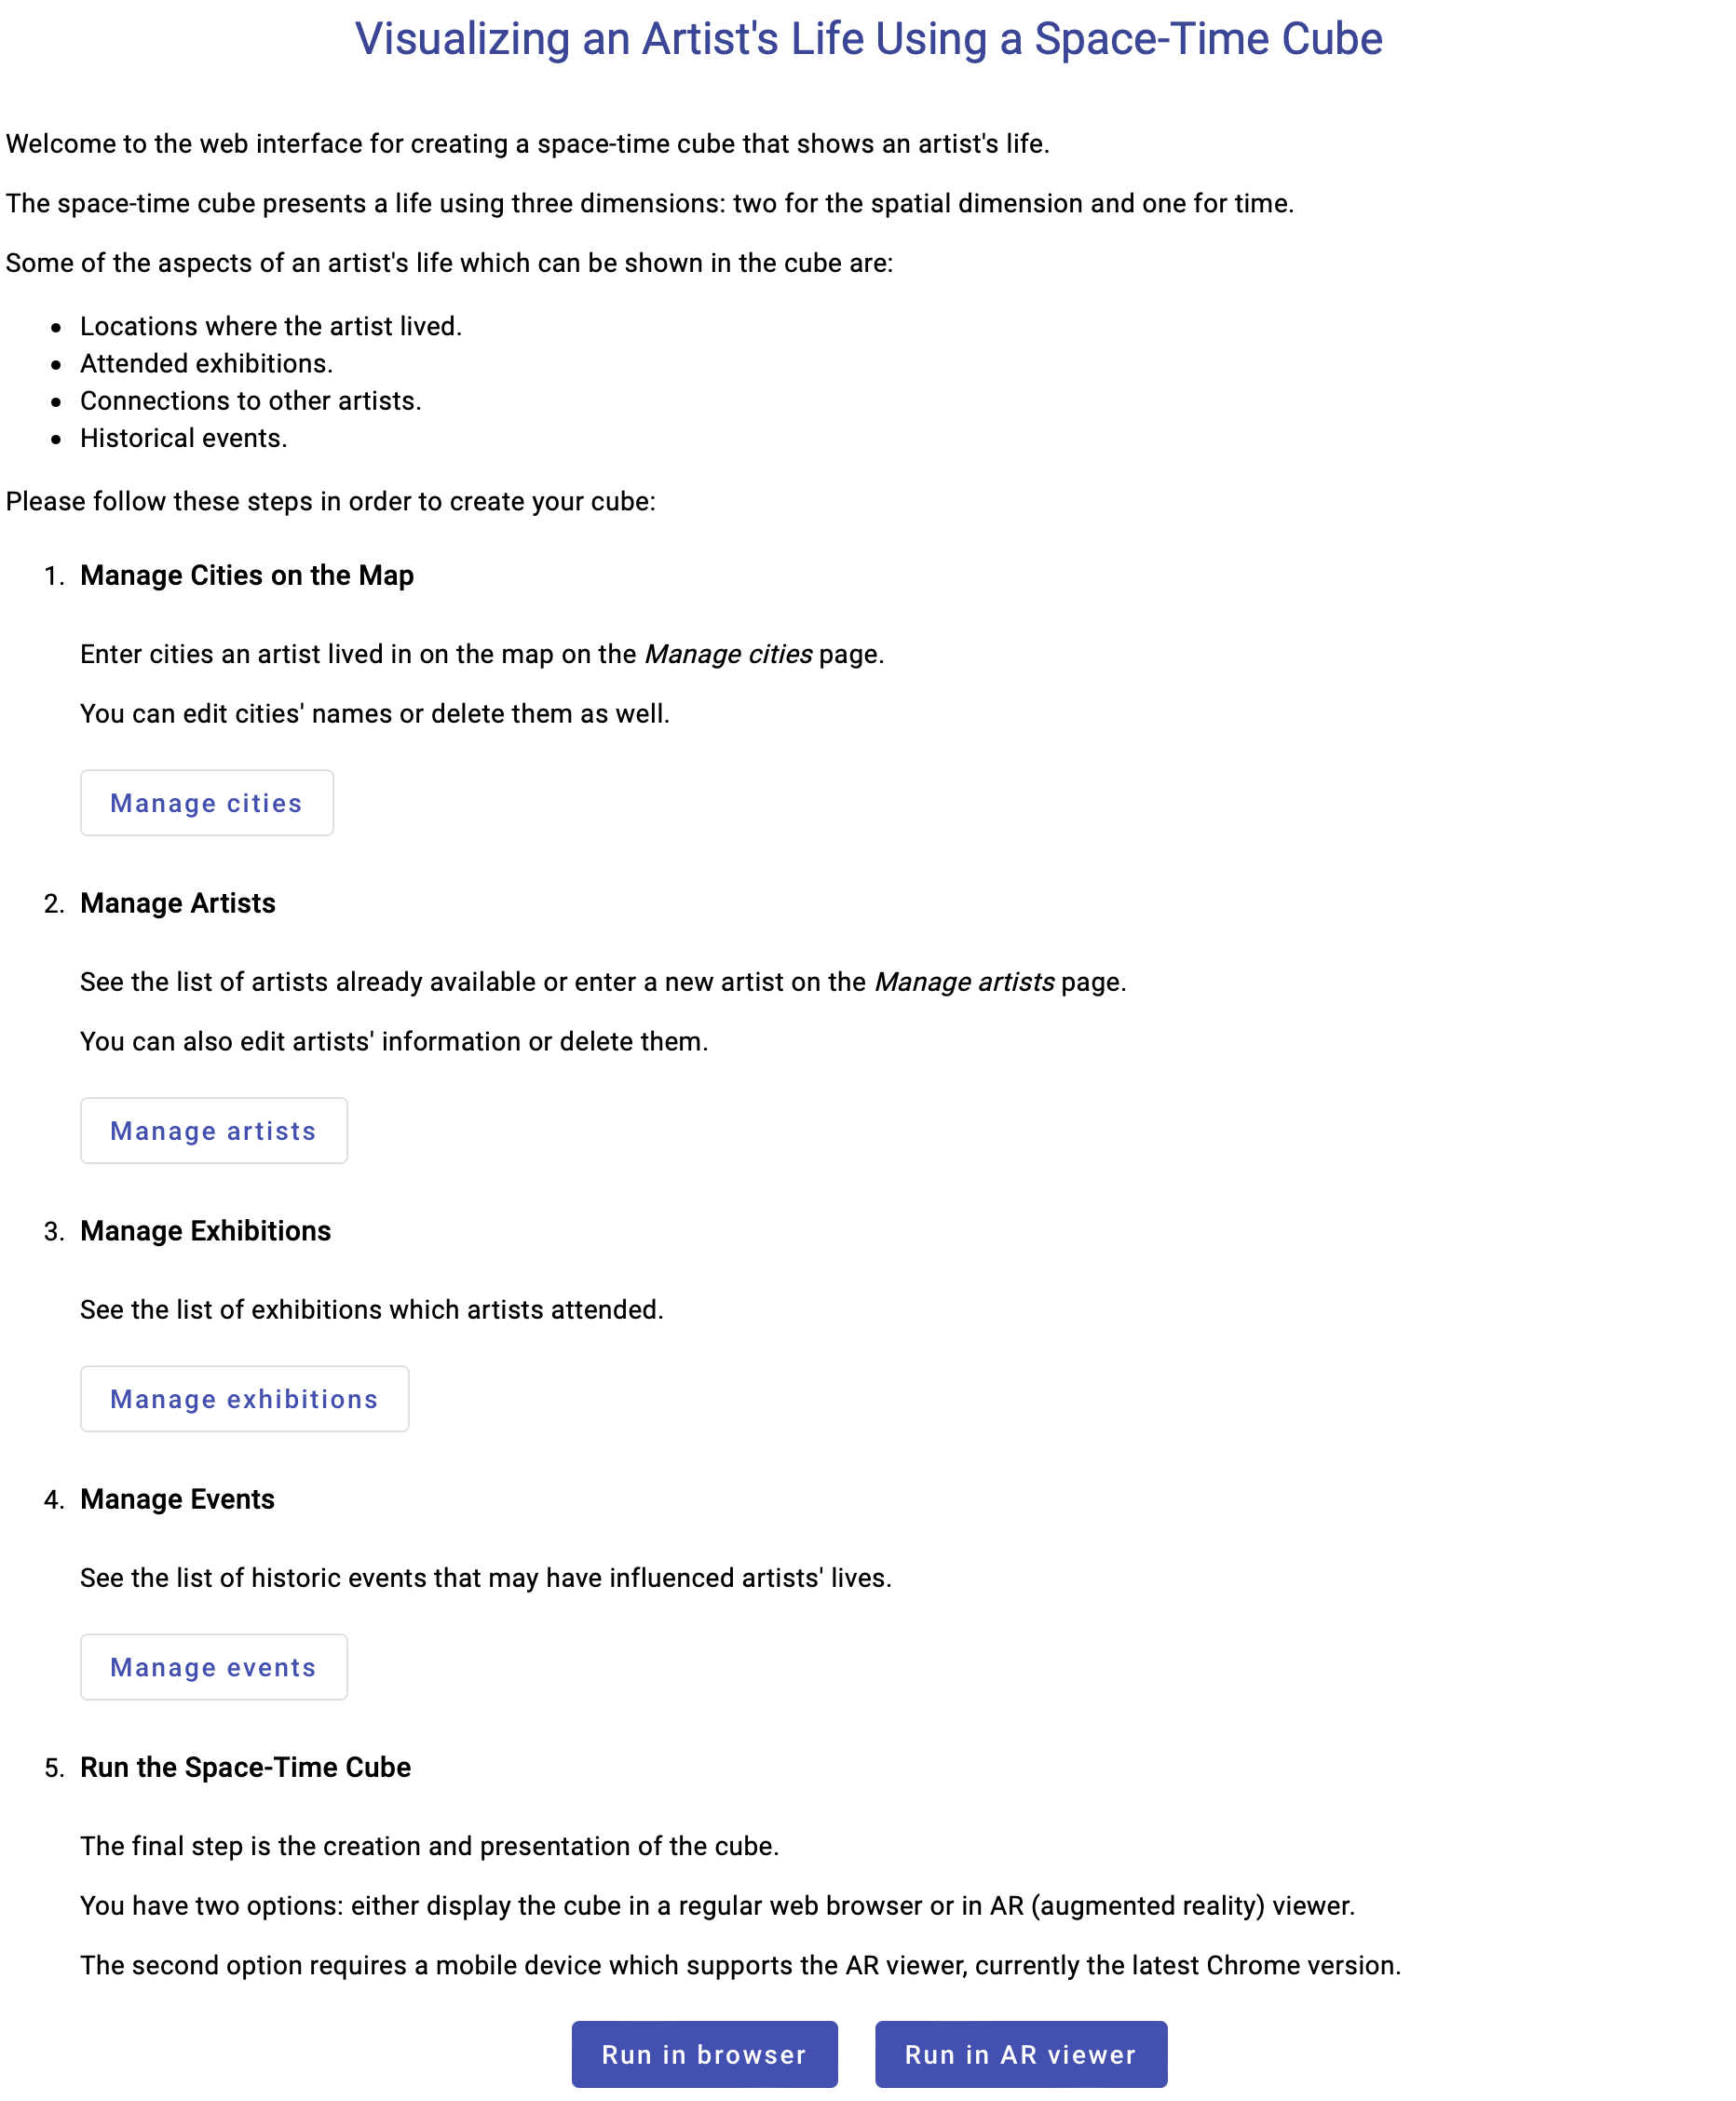
\includegraphics[width=2cm]{graphics/1}
        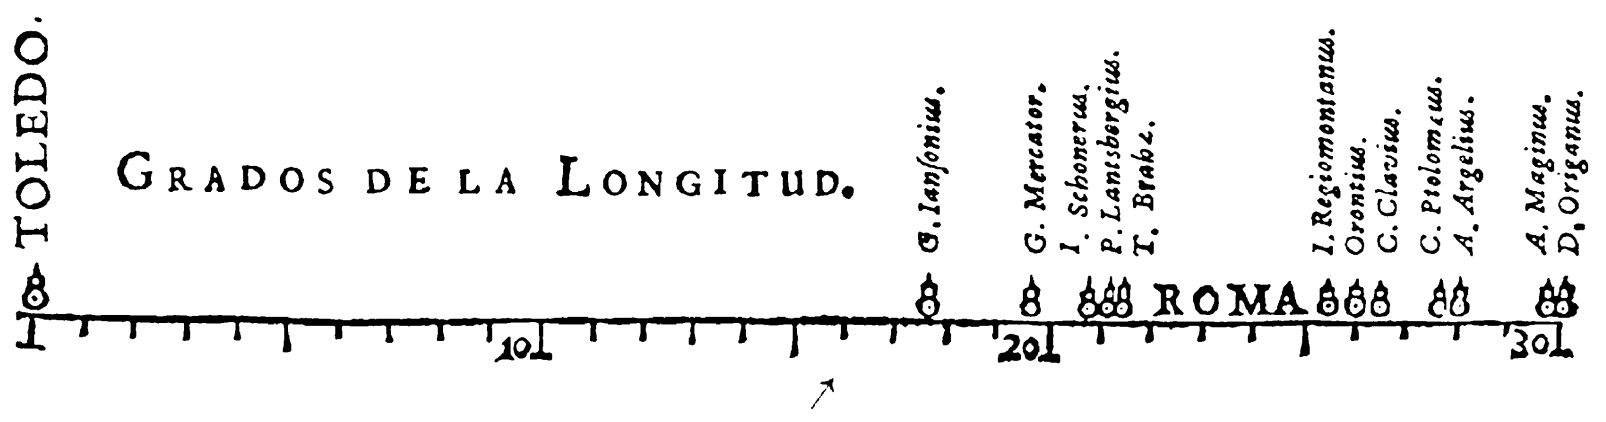
\includegraphics[width=\textwidth]{graphics/2-literature-review/1}
    \end{center}
    \caption{van Langren's 1644 graph of longitudes between Toledo and Rome~\citep{friendly2010first}}
    \label{fig:figure2.1}
\end{figure}

Other two important examples in the history of data visualization from the 19th century are Napoleon’s March Map
by Charles Joseph Minard and the Broad  Street Cholera Outbreak Map by John Snow. Napoleon’s March Map was described as
potentially the best statistical graphic ever drawn~\citep{tufte2001visual}.

The map shown in~\Cref{fig:figure2.2}, called the Sankey diagram nowadays, shows Napoleon’s huge losses during
his invasion of Russia in 1812. The army counted 422,000 soldiers at the beginning of the march, as indicated by the
thickness of the beige line, and managed to enter Russia with only 100,000 of them. The return to Poland was even more
disastrous, as shown by the lower black band, where most of the soldiers froze because of the cold winter. Only 10,000
men returned. Besides the army’s size and temperature, the map also shows its locations and movement direction.

\clearpage

\begin{figure}[h]
    \begin{center}
        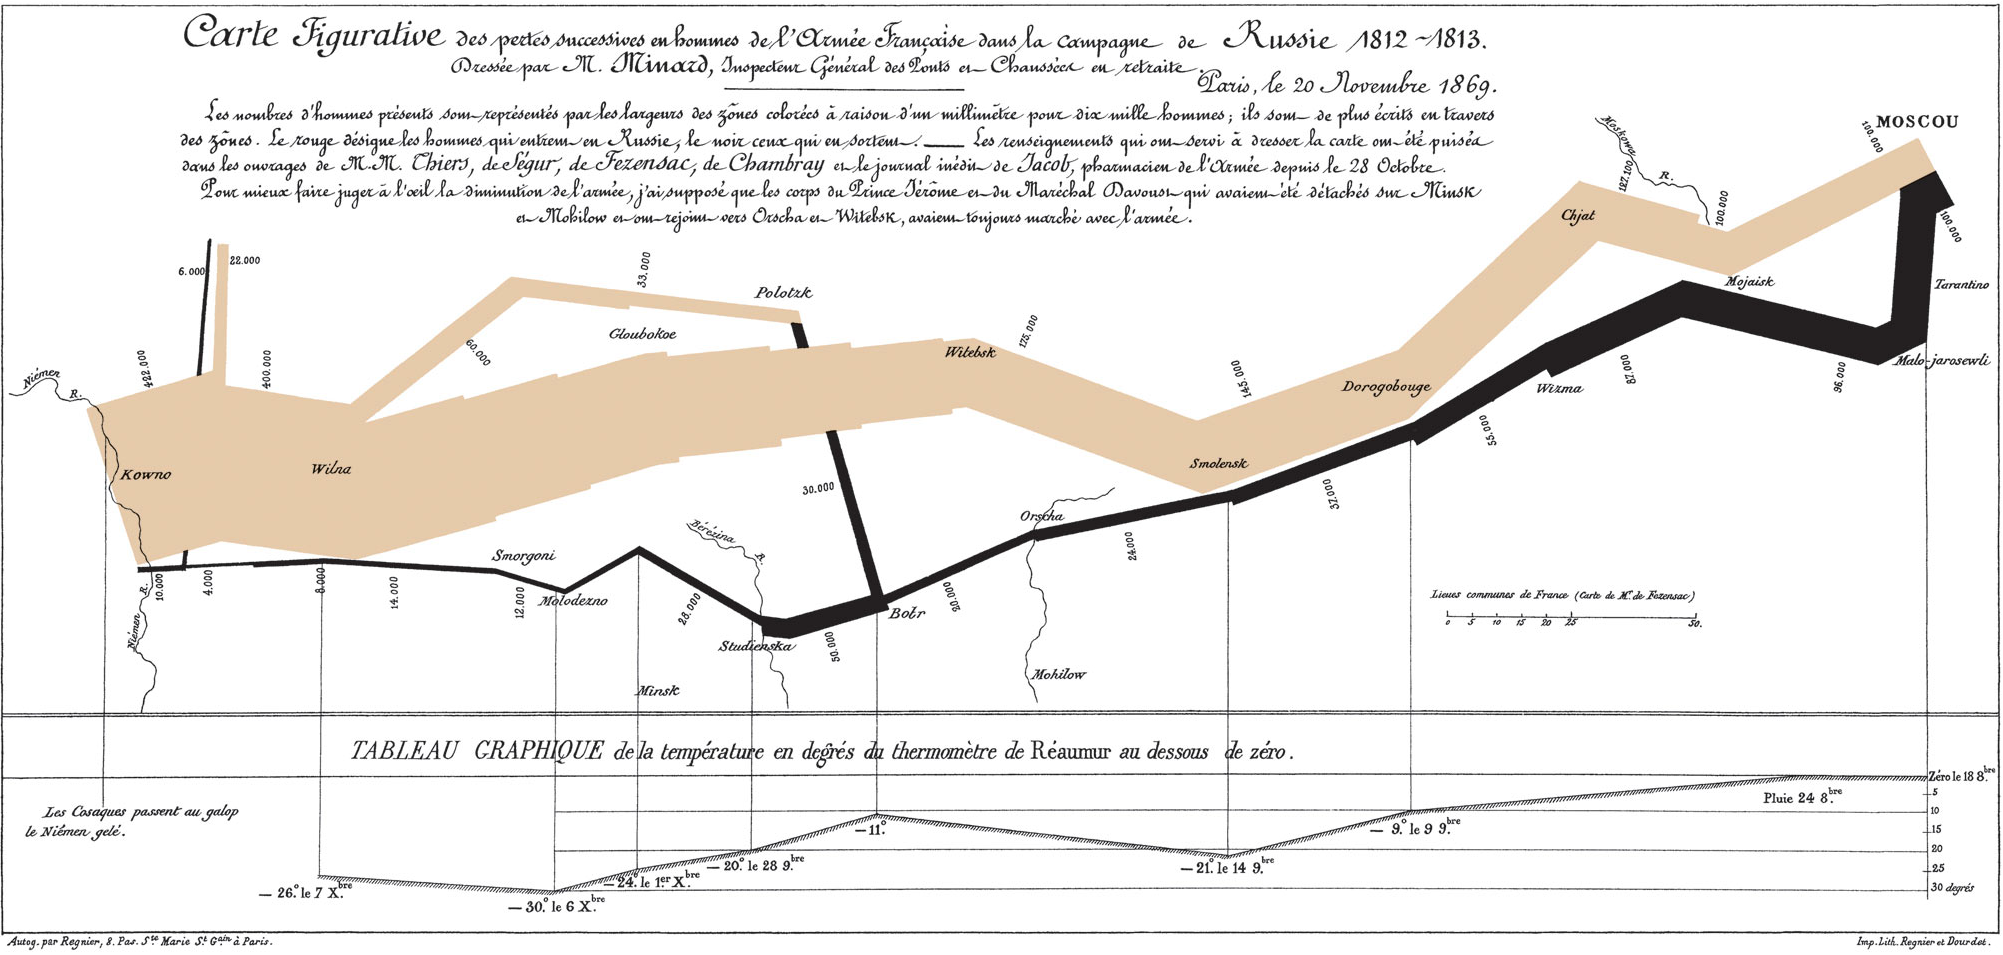
\includegraphics[width=\textwidth]{graphics/2-literature-review/2}
    \end{center}
    \caption{Napoleon’s March Map by Charles Joseph Minard~\citep{corbett2001charles}}
    \label{fig:figure2.2}
\end{figure}

\begin{figure}[hbt!]
    \begin{center}
        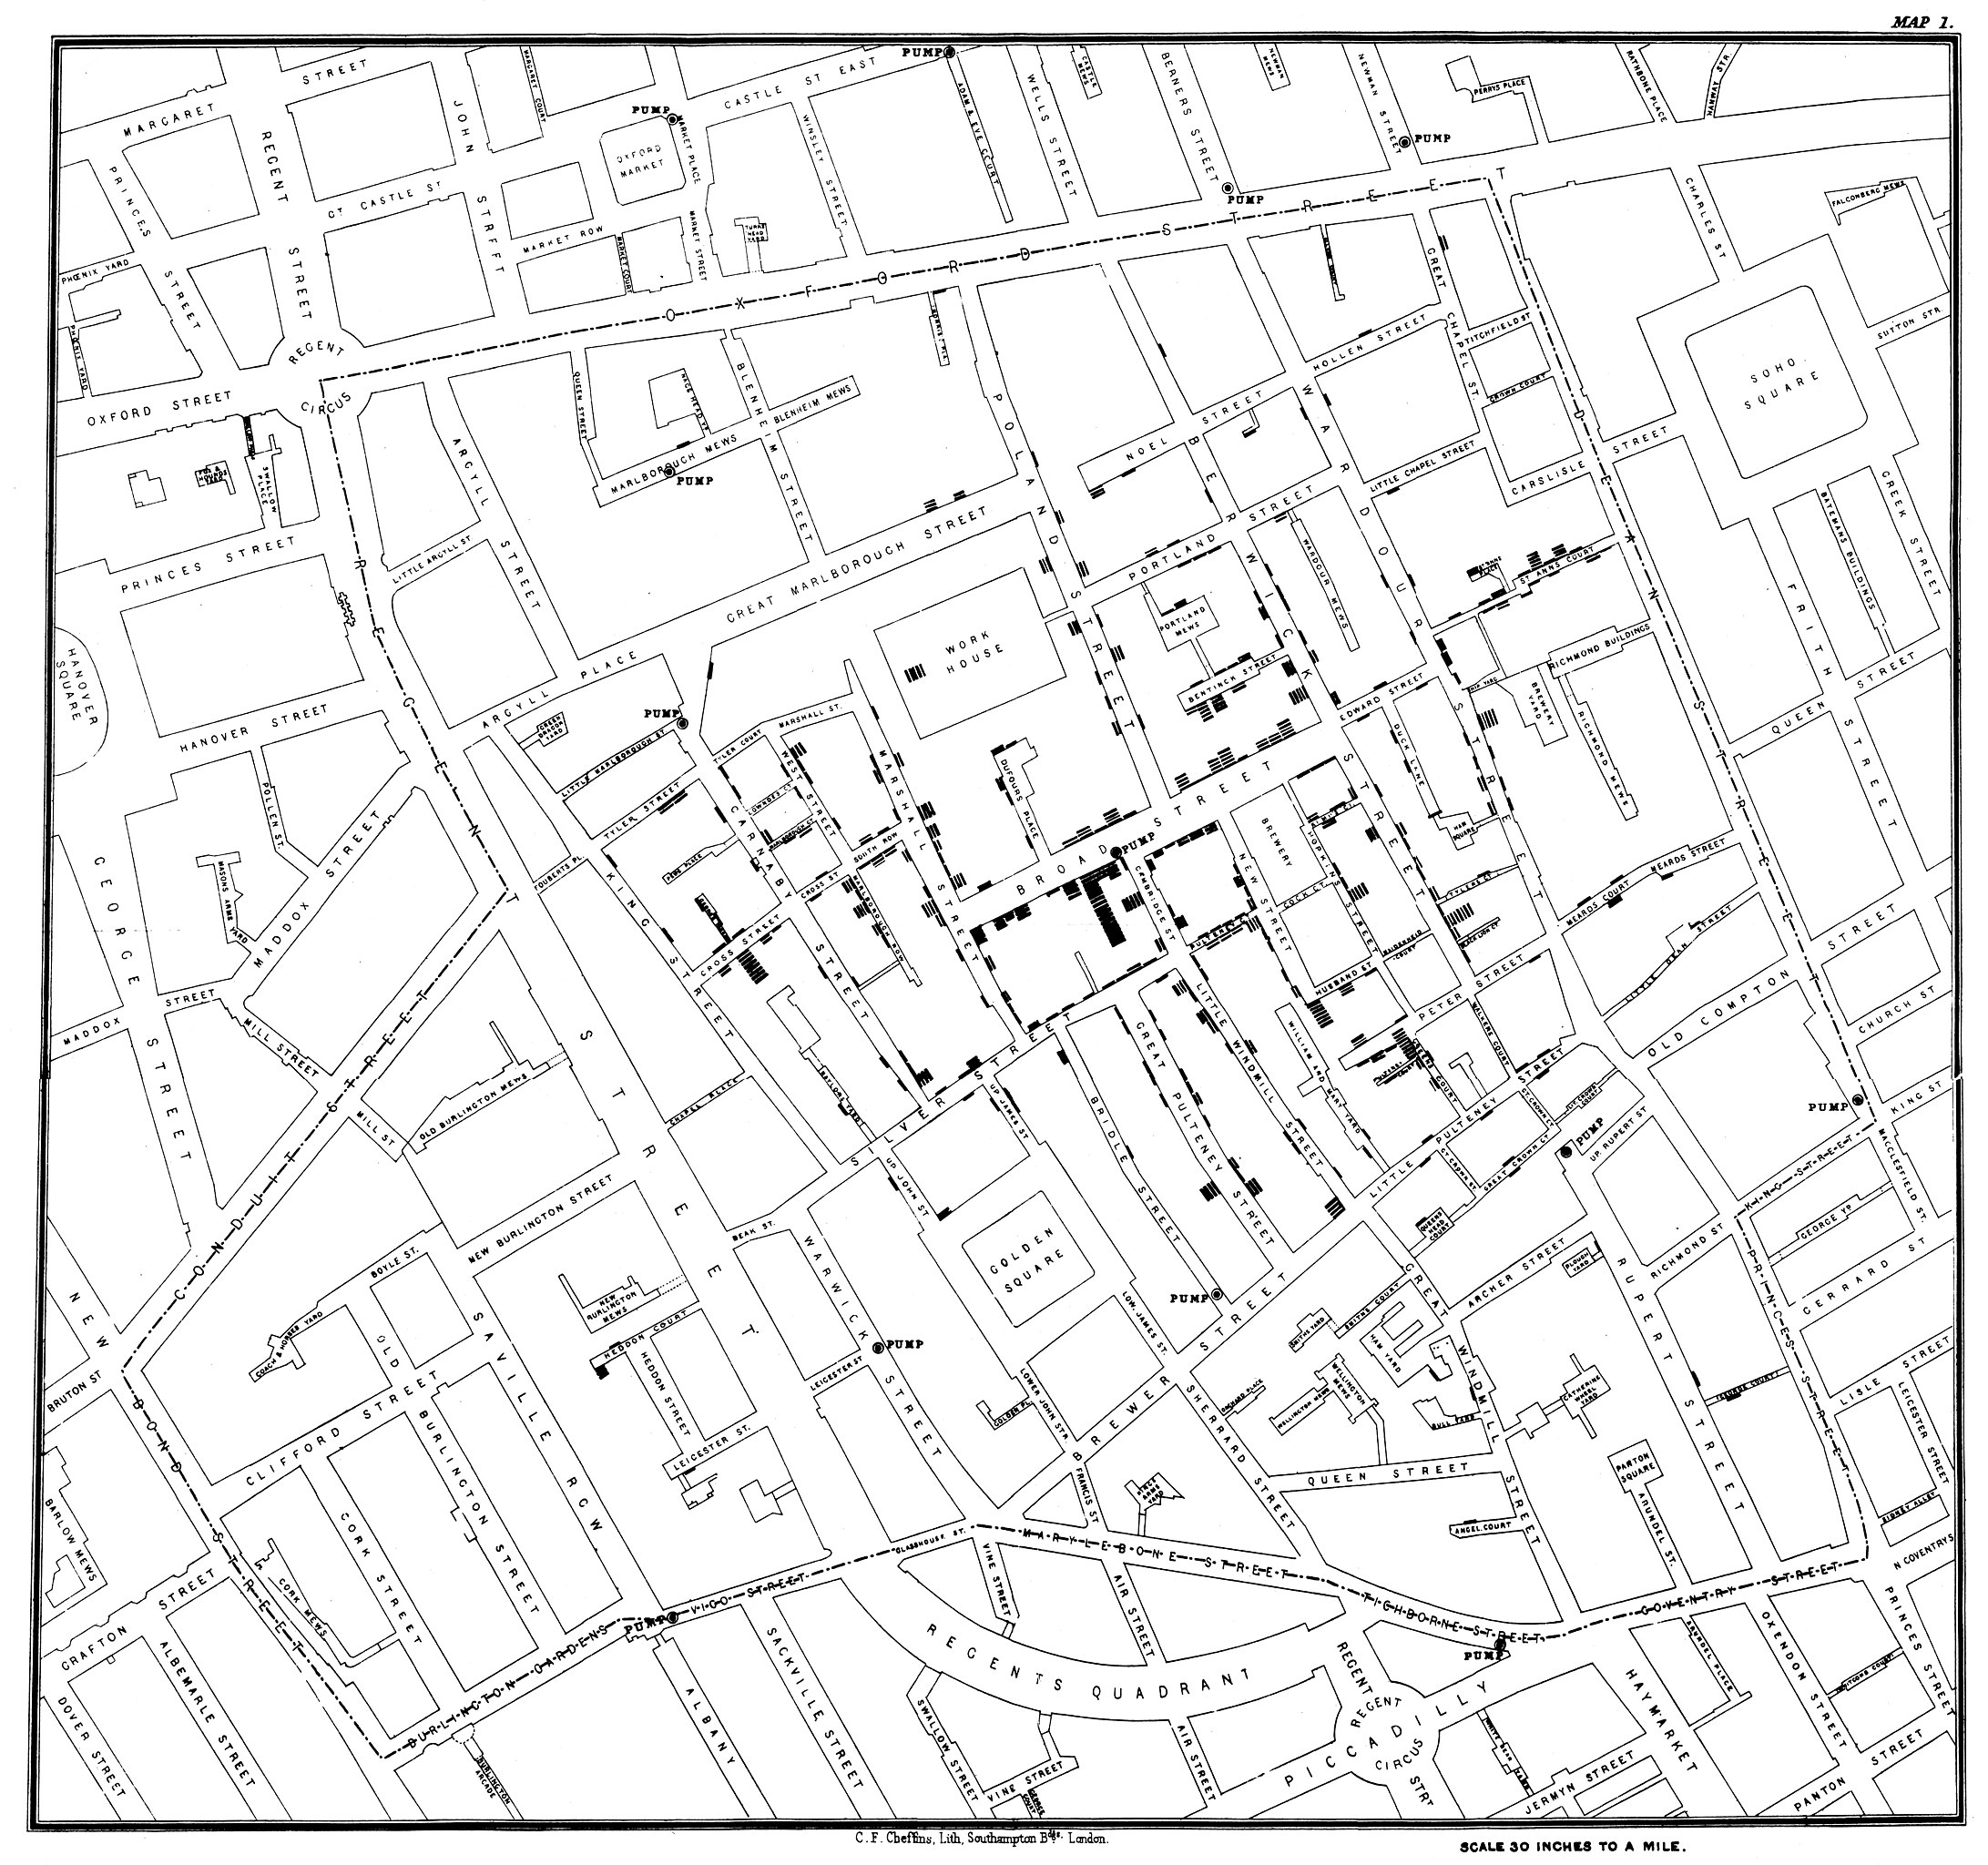
\includegraphics[width=0.7\textwidth]{graphics/2-literature-review/3}
    \end{center}
    \caption{Cholera Outbreak Map by John Snow~\citep{snow1855mode}}
    \label{fig:figure2.3}
\end{figure}

\clearpage

The second example is the Cholera Outbreak map in Broad Street, London. As seen in \Cref{fig:figure2.3},
John Snow, an English physician, marked each death caused by cholera using a small bar. They stacked into rectangles as the number of deaths
increased. The goal of the map was to try to understand the reason behind so many deaths in this particular area
of London. Snow later discovered that the households were all using the same water pump placed in the middle of
Broad Street, which was contaminated by sewage~\citep{snow1855mode}.

The last example worth mentioning is the one by Florence Nightingale. The rose diagram called Diagram of the Causes of
Mortality in the Army of East represented the mortality of the British Army in the Crimean War from April 1854 to March 1855
(right circle) and April 1855 to March 1856 (left circle).

\begin{figure}[hbt!]
    \begin{center}
        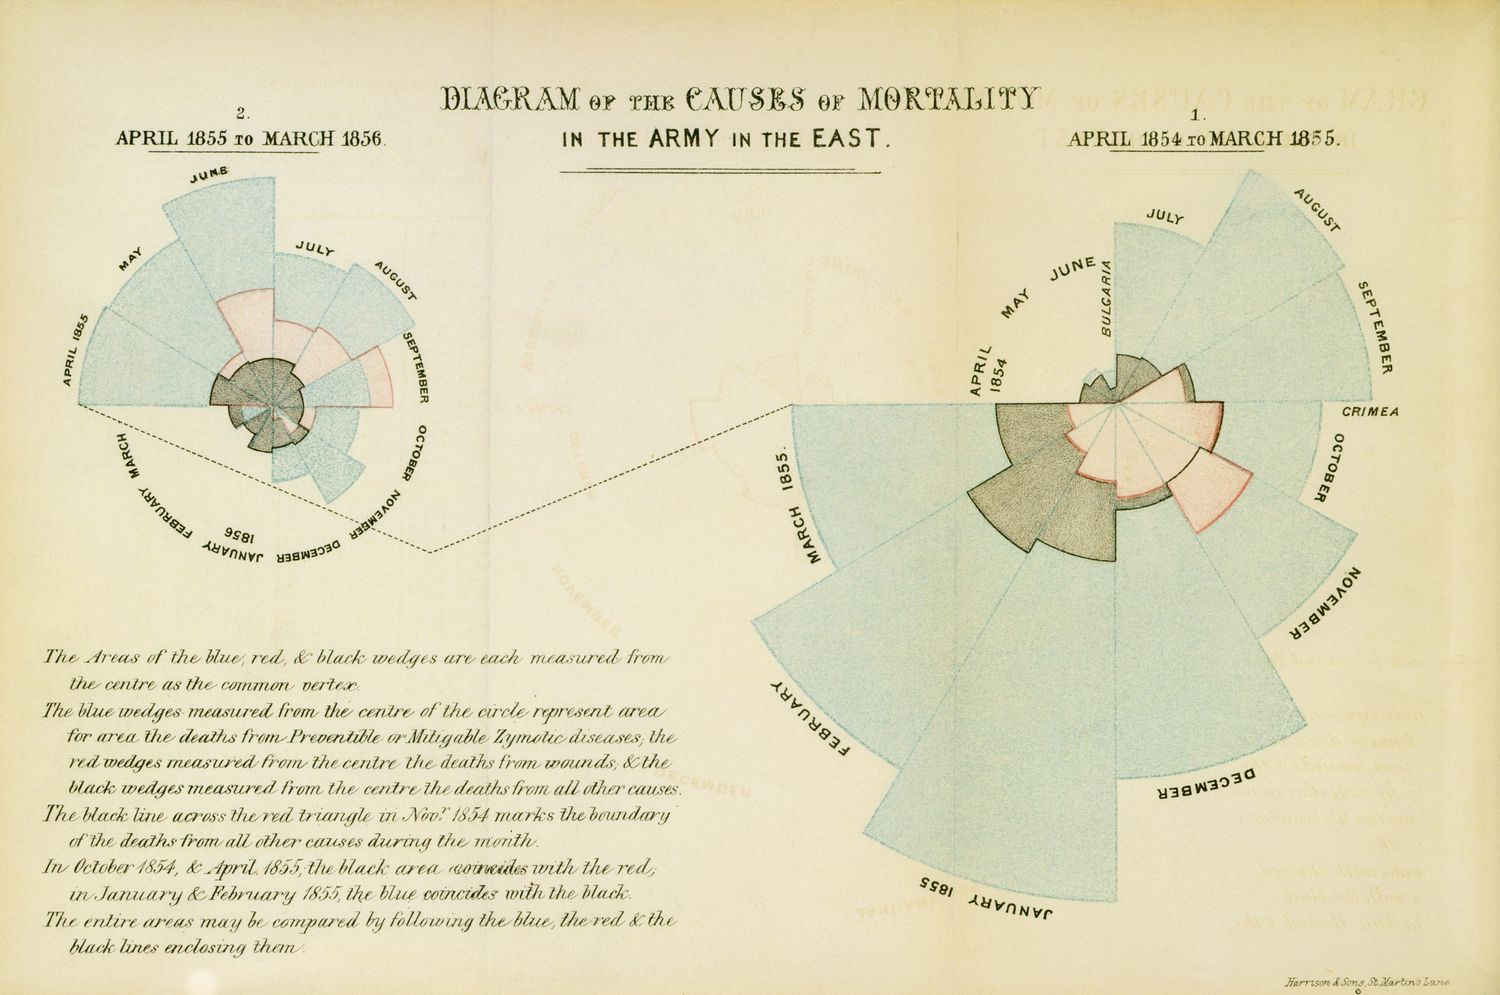
\includegraphics[width=\textwidth]{graphics/2-literature-review/4}
    \end{center}
    \caption{Florence Nightingale's Rose Diagram~\citep{nightingale1858notes}}
    \label{fig:figure2.4}
\end{figure}

Each circle is divided into 12 slices for each month, showing the monthly death rates. As written in the
description, the blue wedge measures the number of deaths from diseases, the red one measures the deaths from wounds,
and the black one measures deaths from other causes. We can see from the graph that at that time, the main reason for so many deaths
was not the actual war, but the diseases soldiers had which were preventable, but unfortunately lethal for them. This
led to the improvement of hospital hygiene, and overall, to the decrease in death rates from preventable diseases~\citep{nightingale1859notes}.
